\section{Main Result}
This chapter provides a detailed description of the process through which the proposed system has been created. Starting from the requirements elicitation process up to the implementation and testing phases, the step by step workflow of the project is reported in the following sections.

\subsection{System Analysis and Planning}
The scope of this project is to develop a platform that provides customisable software products tailored for correlating vendors and customers in the form of both a web platform and a mobile application. To ensure that both the designing and the implementation phases converge to the successful attainment of the project's goals, project management techniques have been applied. As a result, some deliverables have been created to help identify the specific requirements of both the primary and generated systems, as well as to plan and organise the development phase. These deliverables consist of the Conditions of Satisfaction, the Requirements Breakdown Structure, the Work Package Breakdown and the project's development schedule.

\subsubsection{The Scoping Process}
The analysis of the project's scope leads to the identification of the Conditions of Satisfaction, which provide the means of establishing when the project has reached the end stage. The COS outlined for this project are:\\\\
1. A fully-functional solution is generated in less than 10 minutes.\\
2. The customers are provided with two different means of using the system.\\
3. The system customisation options cover most types of vendors.\\\\\\

Having determined the success criteria of the project, the properties of the end system could be established. Derived from the scope of the project, the core functionalities of the system comprise the high-level requirements, which form a necessary and sufficient set for the attainment of the goal \cite{holyer_2016}.\\\\
1. A complete system is delivered based upon specific requirements and features.\\
2. The solution presents a list of offers for the chosen product or service categories based upon distance, rating score or offer value.\\
3. The chosen offer can be purchased and redeemed at the location.\\

This provided a sufficient base for generating an initial Requirements Breakdown Structure. The initial step for identifying the core features of the system was decomposing the high-level requirements into necessary functions and sub-functions. However, due to the complexity and dynamic nature of the end-solution, the set of system requirements has always been adapted throughout the development process. The final form of the Requirements Breakdown Structure is:\\\\
1. A complete system is delivered based upon particular criterion and features.\\
\indent	1.1. A customisation platform is provided to the client.\\
\indent\indent		1.1.1. The client can choose a system based upon location, product or service.\\
\indent\indent		1.1.2. The system must be suitable for offers of different categories.\\
\indent\indent		1.1.2. The client can customise the appearance of the end-system.\\
\indent	1.2. iOS and Web applications, server and database templates are created.\\
\indent\indent		1.2.1. Database templates matching any combination of customisation criteria are designed.\\
\indent\indent		1.2.2. A server component template is created.\\
\indent\indent		1.2.3. An iOS application template is created.\\
\indent\indent		1.2.4. A Web application template is created.\\
\indent	1.3. The necessary and sufficient set of features and functionalities for the generated system are identified.\\
\indent\indent		1.3.1. Any solution provides rating, directions and offer description features.\\
\indent\indent		1.3.2. Product or service based solutions offer the possibility of offer purchasing.\\
\indent\indent		1.3.3. Service based solutions provide an appointment management system.\\
2. The solution presents a list of offers for the chosen product or service categories based upon distance, rating score or offer value.\\
\indent	2.1. An updated list of offers is displayed, specifying the distance from the customer's current position.\\
\indent\indent		2.1.1. The system can locate the customer's current position.\\
\indent\indent		2.1.2. Customers can view all the offers within a 50-kilometre radius.\\
\indent	2.2. The customer can filter the list of offers.\\
\indent\indent		2.2.1. The list can be sorted by proximity, rating score or offer value.\\
\indent\indent		2.2.2. Customers can manage their favourite locations list.\\
3. The preferred offer can be viewed, purchased and redeemed at the location.\\
\indent	3.1. The solution provides details about the vendor and the location.\\
\indent\indent		3.1.1. The customers can view the description, rating mark and available offers for any location.\\
\indent\indent		3.1.2. The system provides directions to the location via GPS or through Augmented Reality.\\
\indent\indent		3.1.3. Customers can provide a rating mark after purchasing an offer.\\
\indent	3.2. Customers can purchase offers with credit and debit cards.\\
\indent\indent		3.2.1. Customers can add credit to their accounts.\\
\indent\indent		3.2.2. The vendors are transferred the value of an offer when purchased.\\
\indent\indent		3.2.3. The customers receive receipts for their purchases.\\

Following this set of requirements ensured the generation of autonomous systems suitable for any product or service. The presentation components provide all the necessary functionalities needed in customers' search for the best-suited offer, as well as a platform for loyalisation by enabling them to select their favourite vendor locations. Also, this Requirements Breakdown Structure helped in identifying the customisation criteria necessary for covering most of a potential client's requests. As a result, a Project Overview Statement was written to record and maintain a reference to the initial decisions for the project.\\

The next step towards identifying the best-suited approach to developing the system was prioritising the Scope Triangle. The scope of the project is the most critical aspect, as it must target the needs of a vast number of both customers and vendors, thus making it prone to revisions. The system's quality is of close importance, as it is essential to acquiring and maintaining a good customer base. Having less than three months for all of the phases of development, the time for creating such an extensive project is short, proving to be the third most critical aspect. Despite that, the priority is developing a comprehensive and reliable system. The resource availability and the cost could turn out to be an issue in the development of a complete solution. However, these aspects are least likely to change as they are outlined from the beginning.\\

\begin{table}[t]
\centering
    \begin{tabular}{ | l | p{1.2cm} | p{1.2cm} | p{1.2cm} | p{1.2cm} | p{1.2cm} |}
    \hline
    Variable / Priority & Critical (1) & (2) & (3) & (4) & Flexible (5) \\ \hline
    Scope & x &  &  &  &  \\ \hline
    Quality &  & x &  &  &  \\ \hline
    Time &  &  & x &  &  \\ \hline
    Cost &  &  &  & x &  \\ \hline
    Resource availability &  &  &  &  & x \\
    \hline
    \end{tabular}
 \caption{Prioritising the Scope Triangle}
\label{tab:scope_triangle}
\end{table}

While the project started with a clear goal, the solution was not yet fully identified at the time. Even though a minimum set of requirements was identified, both the primary and the generated systems were not clearly outlined. Also, further functionalities for such a retail system could and have been identified further on. Based on these factors, the analysis conducted previously, as well as on the importance of the project and the amount of time available, the chosen approach towards developing the systems was the Agile Project Management. Thus, the Adaptive Project Management Life Cycle was adopted, outlining the conclusion of the project's scoping phase. 

\subsubsection{The Planning Process}
Having identified the initial requirements for the system, a project plan was outlined in order to organise the following stages of the development process. This provided a clear roadmap for the sequence of steps that needed to be followed as to minimise uncertainty and increase efficiency. However, as the Adaptive lifecycle was chosen as the PMLC, identifying clear tasks and creating an overall schedule was hindered by the large complexity. The approach to solving this issue and maintaining awareness of the progress and results is described in this section.\\

As the depth of the Requirements Breakdown Structure was not known after the features level, the solution could not be defined yet. Thus, the planning process started with documenting and creating an initial plan using a board and sticky notes. This task provided a good initial approach, as it helped in transforming the features of the RBS into work packages and estimating the duration and complexity of every one of them as can be seen in Figure~\ref{fig:wbs} in the Appendix. This was followed by organising the identified work packages using a software tool to maintain persistency and to enhance the visual aspect of the schedule.\\

Not having an explicit description of the solution, the work packages were arranged into different development phases, following Agile development guidelines \cite{wysocki_2013}. All phases ended with a feedback loop to assess their completion, helping to determine if the next phase could start or if a new cycle of the current step should be launched to shape further the work packages involved. Following this model aided in managing the complexity and uncertainty of the project, every cycle converging to a complete solution. Five development stages were planned, each starting with a partial perception of its expected result and based upon certain assumptions about the input received and completion level of the previous cycles, thus establishing the five major milestones of the project. Aiming both to fulfil already existing tasks and to identify new functionalities for the system resulted in the definition and completion of the end system.\\

\begin{figure}[!ht]
\centering
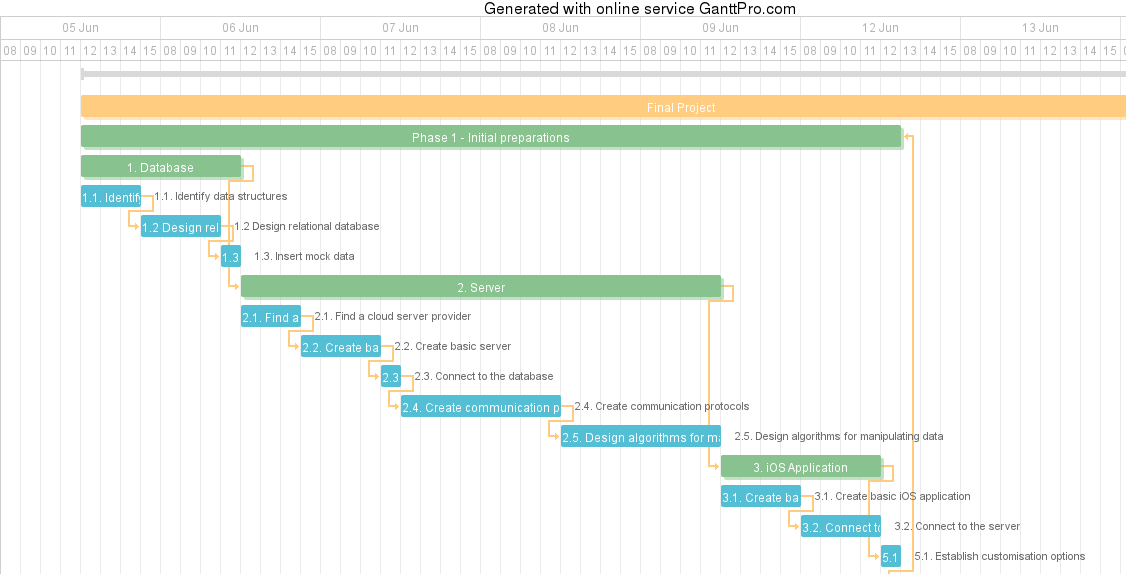
\includegraphics[scale=0.2]{img/phase1.png}
\caption{First phase of the project plan}
\label{fig:phase1}
\end{figure}

The first phase was the most crucial as its primary purpose was to identify and perform the abstraction of all the business entities involved in the system. Also, the data structures had to be defined to start designing a coherent database structure. This was particularly challenging as the elements this system targeted were subjective and based upon customer preferences, so the requirements analysis performed had to be extensive. Further on, the server component had to be designed and implemented as it was responsible for all the generated system's business logic, acting as a middle point between the database and both the iOS and Web clients. The first milestone was considered reached when the server, the database and a rudimentary iOS mobile application were created and the communication between them was functional, these components representing the deliverables of the initial stage.\\

\begin{figure}[!ht]
\centering
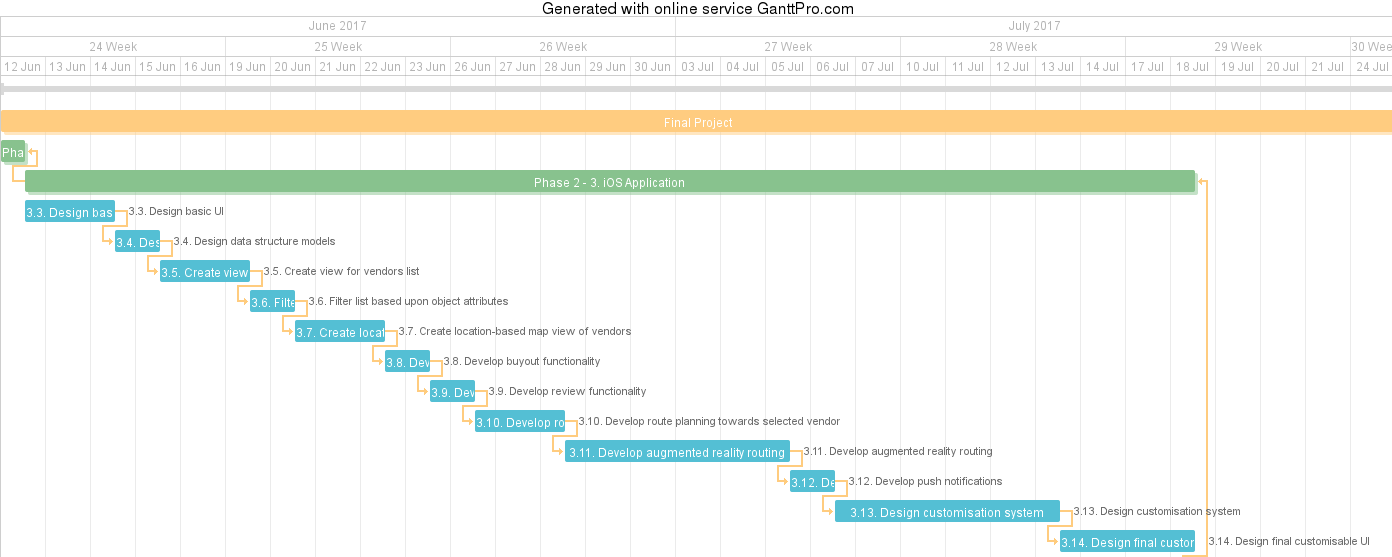
\includegraphics[scale=0.2]{img/phase2.png}
\caption{Second phase of the project plan}
\label{fig:phase2}
\end{figure}

The second phase comprised the work packages related to the iOS application template. The launching of this stage implied that the server was active and that the system's functionalities were already implemented. Thus, the iOS client development stage would revolve around presenting the information received from the server and the specific mobile features of the system. However, this was expected to be a time consuming and of a high importance process as this component is the main interaction point with potential customers. Also, the augmented reality feature increased the level of uncertainty for this cycle. The deliverable of this phase was a fully functional iOS mobile application template, upon the completion of which the second milestone was considered to be reached.\\

The third phase of the project schedule (Figure~\ref{fig:phase3} in the Appendix) plans the work packages responsible for the creation of the Web application and the generation platform. This stage was expected to be less complicated than the iOS application development, as some features were not included in this client platform, because they had to make use of particular hardware functionalities not available to a browser, such as geometric sensors and video camera usage. However, the primary generation system proved to be more complex than expected, requiring an extra cycle for the completion of this phase. The milestone was reached when all of the established features were implemented, the deliverable being a functional client Web interface template and a generation system.\\

The fourth and fifth phases (Figure~\ref{fig:phase4} in the Appendix) consisted of deploying, debugging and testing the overall system, thus being dependent on the deliverables from the previous cycles. Extra time was allocated for each work package involved, as neither of the components was yet extensively tested. Thus, a time margin was granted for fixing any system or logic issue that became visible. Reaching the milestone of the fifth stage implied that the project's solution was identified and created, this being asserted by evaluating the system based upon the success criteria of the Conditions of Satisfaction.

\subsection{System Design}
As an Agile project, the functionalities, features and even requirements may change throughout the development process. To increase the efficiency and reliability of the software solution, Model Driven Development has been chosen as the primary approach for designing and implementing both the main and generated systems. Through model creation and transformation, the complexity of the project will be reduced. As the initial step towards developing the solution is the abstraction of the components and interactions, this will aid in maintaining the core functionalities throughout the usage of multiple types of programming languages, as well as in the case of changing an already used technology. Also, following MDD techniques provides clear steps in case of changing or reusing the components involved \cite{lano_2009}. This section aims to present the steps taken for outlining the resulted overall system design.\\

The first step towards identifying and defining the main functionalities and components of the system is to create a Platform Independent Model. The system model regarding the core domain notions and software independent structures helps to convey the high-level functionalities of the system, as well as provide flexibility and reusability across both the iOS and the Web platforms. This has been achieved by outlining the Business Concept Model based upon the business requirements identified in the previous section, in addition to the system requirements resulted from establishing the Use Cases for the two systems described by this project \cite{sastry_2017}. The Unified Model Language was chosen to present the elements of all the design and architecture components of this project.

\subsubsection{Use Cases}

In order to identify the expected system actions and the dynamic behaviour it must have, some Use Cases have been drafted and linked in a Use Case Diagram. This lead to a more in depth understanding of what the sequences of actions should be, thus giving insight for outlining the system's event processing order. This step also provided the means to recognise the actors involved in the usage of the solution, being able to tailor the functionalities based on their positive experience. Through this process, an overview of the components' workflows was able to be identified, providing the sequence of steps needed to ensure a successful interaction. The most important Use Case scenarios have been described in detail in this section to further establish the system's functionalities and requirements.\\

\begin{figure}[!ht]
\centering
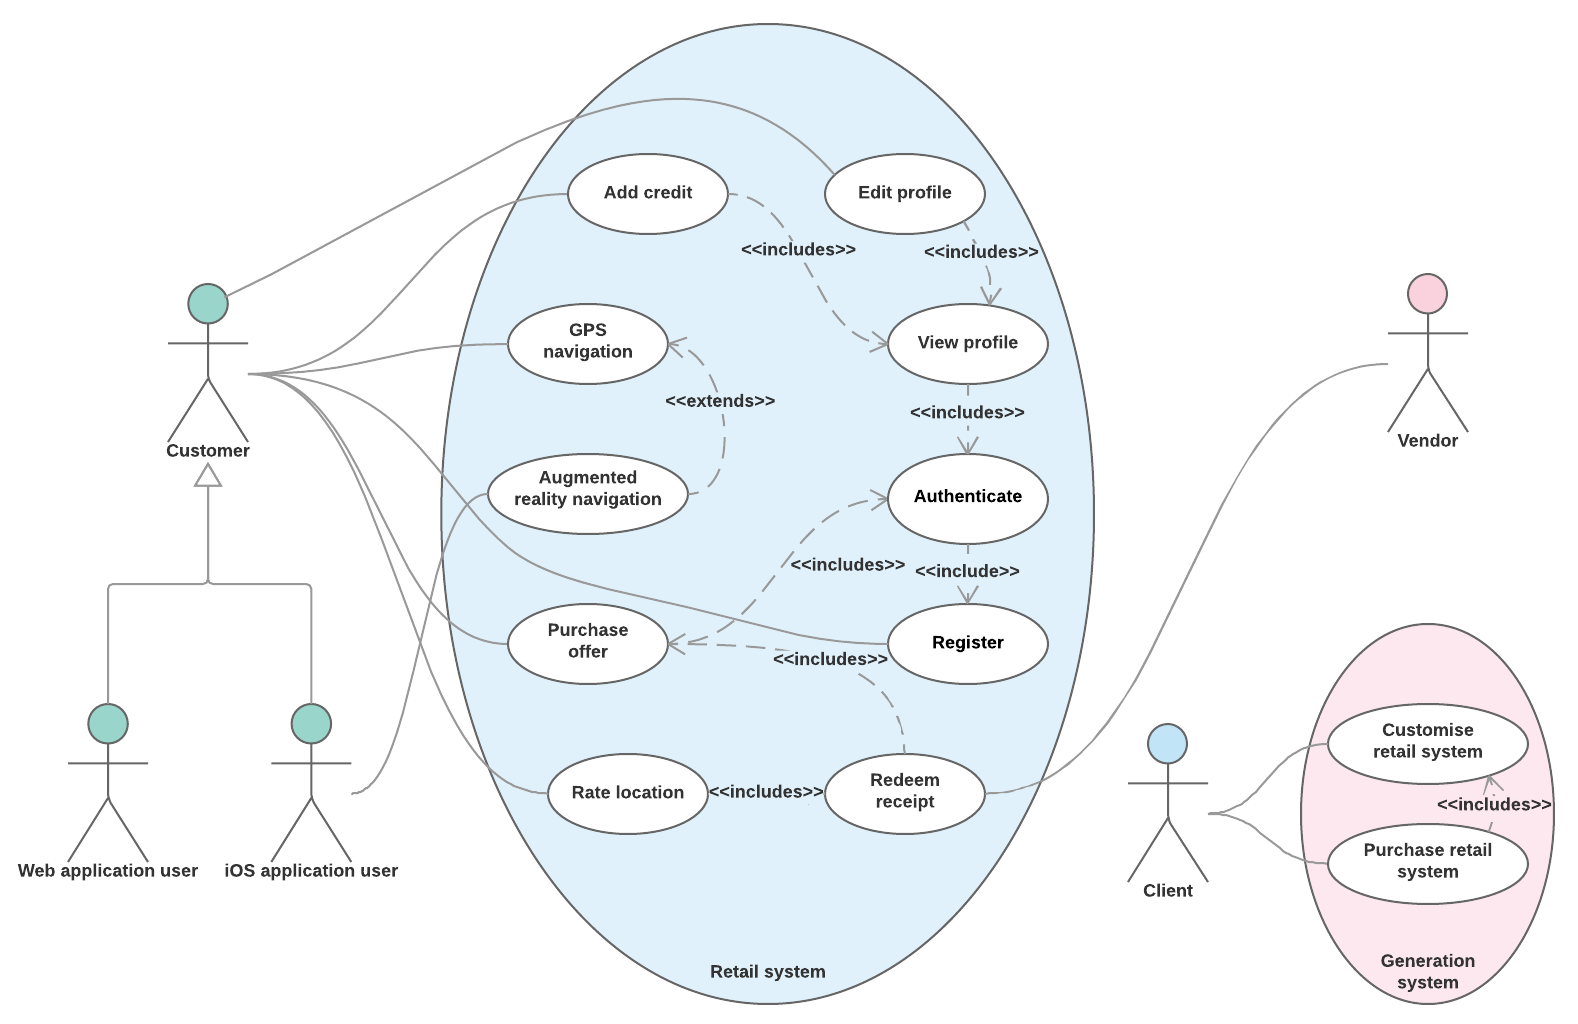
\includegraphics[scale=0.2]{img/Use_Case_diagrams.png}
\caption{Use Case diagrams for the main and generated systems}
\label{fig:use_case_diagrams}
\end{figure}

As seen in Figure~\ref{fig:use_case_diagrams} , the generation system has two primary Use Cases for the interaction with the potential clients, which are abstracted into the Client actor. Following the scenarios of the two cases provides the necessary steps for which a solution can be customised and generated successfully, thus comprising the guidelines for using the main program. The user must first pass through the 'Customise retail system' use case, in which all the generated retail logic components and customisation options must be defined. These include the name of the solution, some classification parameters such as the targeted type of vendors and offer categorising, as well as the colours of the visual elements. The 'Purchase retail system' case uses the client's preferences as input to generate a complete solution and provide the download links for it. This can only be done after the user provides a valid form of payment and the transaction is complete. Thus, this use case includes the first one, forming together the necessary set of steps for the usage of this project's main system.\\

Most of the success criteria and requirements identified in the scoping process concern the generated solution, as it represents the deliverable for the transactions with potential clients and is the main element that provides business value. It's complexity implied a larger number of functionalities, thus leading to multiple use case scenarios for potential customers. The actors identified for the interaction with the system are the customers and the vendors. As there are two different platforms of interaction, the customer agent can be either a web or an iOS application user, both having a large common base of functionalities to use. However, as the mobile application is the main platform, the iOS user has more features at his disposal, such as augmented reality navigation. Also, taking into account the reliability of the system and maintaining a logical sequence of activities in the user interaction, most use cases depend on the successful completion of the sequences of steps stated in other scenarios.\\

This applies to the 'Authenticate' use case among others. The system verifies the credentials entered by the customer actor and either grants access to the application functionalities or alerts the user that access is denied. However, a successful pass through this scenario is based on the completion of the 'Register' use case beforehand. Thus, only by creating an account will the system be able to identify the actor as a user with the necessary permissions. This is only part of the sequence of steps needed to undergo to use the platforms, as the 'Authenticate' scenario is included in most of the others.\\

Adding credit to an existing account implies that a customer has already authenticated, this use case regarding both types of users. The topping up process is of high importance for the system as it is required for the purchasing of offers, the primary revenue source of the vendors and the potential clients. Thus, a scenario has been outlined in order to establish the required steps for customers to credit their account successfully.\\

\noindent 'Add Credit' success scenario:\\
\indent 1. Customer accesses the profile page (having authenticated beforehand)\\
\indent 2. Customer selects to add credit\\
\indent 3. Customer enters the desired amount\\
\indent 4. Customer enters card credentials\\
\indent 5. System authorises the crediting\\
\indent 6. System alerts customer of the successful transaction\\
\indent 7. System credits the customer's account\\
Extensions:\\
\indent 5b. System rejects the transfer\\
\indent\indent 4b.1. Customer may reenter the card credentials or may cancel\\

One of the most important scenarios for the attainment of the project requirements is the successful completion of a purchasing and redeeming cycle. This sequence of actions ends with the vendor actor proceeding with claiming a valid receipt. However, there are a number of successive use cases included in this process. After the authentication, the next important step is to undergo the 'Purchase offer' scenario:\\

\noindent 'Purchase Offer' success scenario:\\
\indent 1. Customer authenticates\\
\indent 2. Customer browses the offers and selects a location\\
\indent 3. System provides appointment intervals (service based vendors)
\indent 4. Customer chooses an appointment interval (service based vendors)\\
\indent 5. System authorises the purchase\\
\indent 6. System provides an electronic receipt\\
Extensions:\\
\indent 5b. System rejects the purchase\\
\indent\indent 5b.1. Customer may add credit or may cancel\\

The last step for redeeming a receipt can only be initiated by an iOS application user, as an initial requirement of the system and as the web component is dedicated to desktop users for the initial version. Thus, after a customer purchases an offer, he is expected to redeem it at the selected location in between the established hours (either between the location's hours for the product based solution or in the appointment interval selected for the service based systems). The main actor in redeeming a receipt is the vendor, as by doing it personally is the only way to ensure that each offer is checked out only once.\\

\noindent 'Redeem Receipt' success scenario:\\
\indent 1. Vendor presses the receipt button\\
\indent 2. System asks for confirmation\\
\indent 3. Vendor provides confirmation\\
\indent 4. System verifies the receipt's validity\\
\indent 5. System approves the redeeming of the receipt\\
\indent 6. Vendor provides the service or product implied\\

One of the most exciting features of the iOS application is the augmented reality navigation. The system calculates the distance to the selected location and provides step by step directions using the iOS device's video camera. The only actor that initiates this use case is the iOS application user, as this functionality depends on precise measurements provided by mobile devices. However, this scenario extends the 'GPS navigation' use case, which is available to both types of customers. The scenario is considered to be successful when the actor arrives at the selected destination.\\

\indent 'GPS Navigation' success scenario:\\
\indent 1. Customer authenticates\\
\indent 2. Customer presses the navigation button\\
\indent 3. System presents the options of providing directions\\
\indent 4. Customer selects navigation via maps\\
\indent 5. System presents a map with step by step directions toward the destination\\
\indent 6. Customer follows the directions until the arrival at the end point\\
Extensions:\\
\indent 4a. Customer selects the 'Augmented reality navigation' scenario:\\
\indent\indent 4a.1. System opens the camera with labels for the step by step directions\\
\indent\indent  4a.2. Customer follows the directions shown on the camera overlay\\
\indent\indent  4a.3. System shows an alert upon the arrival and closes the camera

\subsubsection{Business Type Model}

Identifying the core elements is important as the system will be further shaped based upon them. As a result, some steps have been covered to ensure that the resulting component design is reliable, first being to gather all the elements involved in the lifecycle of the solution and to outline the relationships and dependencies between them. The representations of the domain elements and the associations between them formed the Business Concept Model, an initial design of the entities used and handled in the business area that this system tackles (Figure~\ref{fig:business_concept_model} in the Appendix).\\

As the project aims to develop a customisable solution, both the primary and the generation systems had to be analysed separately. The abstraction of the main component's elements resulted in a set formed of the potential clients, the main system, the customised solution with different possible types and the orders placed for them. Contrary to the reduced complexity of the generation platform's business domain, the group of elements that comprise the custom system's field of interaction proved to be very extensive, covering elements from the types of vendors and offers to the connections with the customers.\\  

The next step in refining the business entities was to classify the elements of the Business Concept Model by identifying what components are of a core, dependent or the category type. This task aimed to distinguish the sections which correspond to primary business information, thus forming the starting point of the component identification process. The method used to differentiate them was analysing which were standalone entities and which were coherent only through their relationship with others. The latter could then be split by checking if they provided means of categorising the main elements or just depended on them. The resulted model for the proposed generated system is presented in Figure~\ref{fig:business_type_model}.\\

\begin{figure}[!ht]
\centering
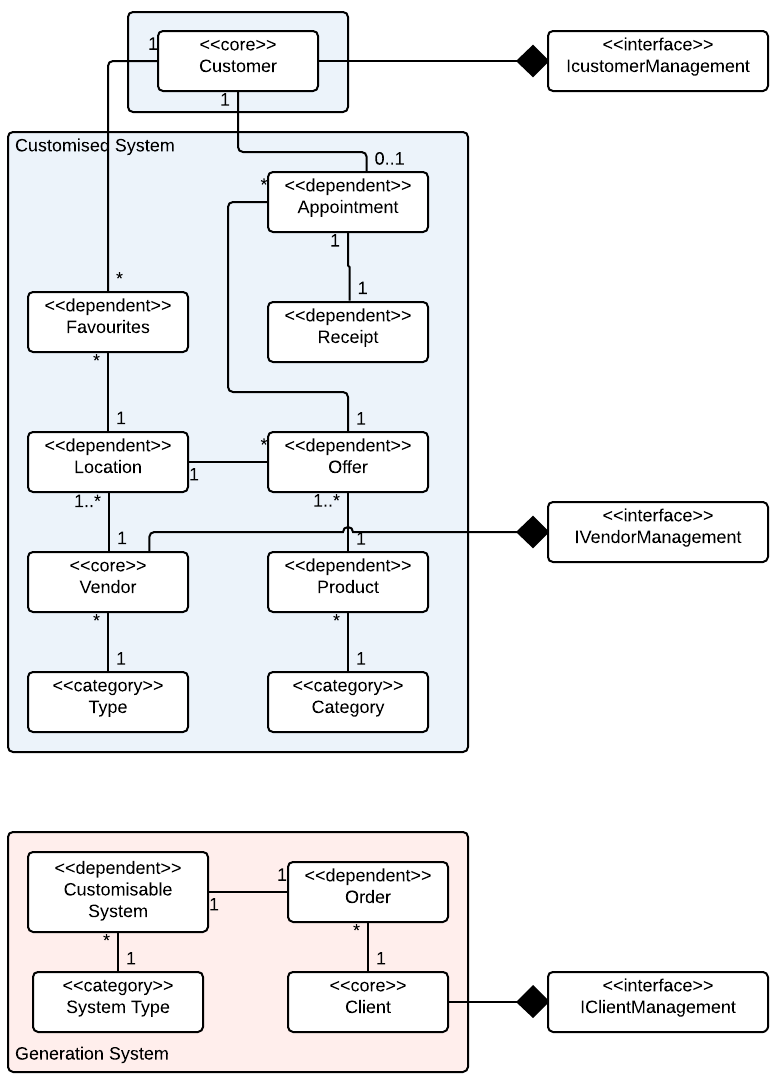
\includegraphics[scale=0.3]{img/Business_Type_Model.png}
\caption{Business Type Model with Business Interfaces}
\label{fig:business_type_model}
\end{figure}

The single core entity of the generation component was found to be the Client. The System Type was easily identified as belonging to the category type, while the Customisable System depended on the Order piece, which in turn depended on the Client. Similarly, the customised template system was comprised of two core elements, the Customer and the Vendor segments, while the others were found to be related to the latter. The Category component provides classification criteria for the Product element, in the same way as Type is a category entity for the Vendor core segment. The rest were identified as dependent types for either the main items or for each other.\\

\subsubsection{Component Identification}
The acquired data obtained through the abstraction of the business elements and the system functionalities identified through formulating the use cases could then be used to model an initial overview of the system's architecture. However, the components that comprise it needed to be defined and the communication interfaces established. In accordance to software design and architecture guidelines, the dependent and category types of the business model belonged to a span of responsibility of the core types. As a result, the interaction points through which these elements could be accessed would be via the core elements, resulting in the identification of these regions as the system's business components and their access points as the business interfaces \cite{hamza_2017}. The resulting business components are the Customer and the VendorManagement elements with the ICustomerManagement and IVendorManagement interfaces as can be seen in Figure~\ref{fig:business_type_model} in the Appendix. The operations present for the business interfaces are the descriptions of the interaction between the business and system components.\\

Following the same set of design rules, the system interaction with the business elements would be achieved through interfaces resulted from the system's behaviour in the use cases, with the limit of one such interface per every primary use case. In consequence, the system would form a single component with multiple interaction points. The identified system interfaces can be seen in Figure~\ref{fig:system_interfaces}. Analysing the use case of the generation component lead to the decision that its only interface would be the IGenerate communication point, which provided the means of customising a solution and deploying it. Seven different interfaces were thus identified for the retail system, the first of which being the IAuthenticate terminal in charge of checking credentials and creating new accounts operations. IEditProfile would be responsible for presenting and managing user profile details, IAddCredit would provide the crediting authorisation and updating, and INavigate would show the directions based on different settings, as well as handle the augmented reality navigation. The IPurchase and IRedeem interfaces would be responsible for the managing and redeeming of offers and the IRateLocation with the feedback operations.\\\\

\begin{figure}[!ht]
\centering
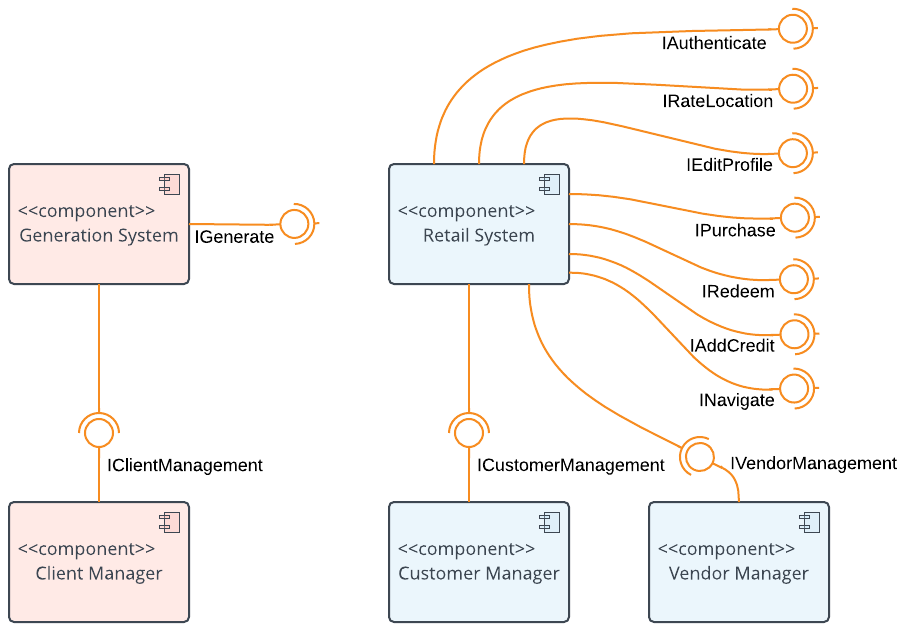
\includegraphics[scale=0.31]{img/Initial_Architecture.png}
\caption{System Interfaces}
\label{fig:initial_architecture}
\end{figure}

Having identified and designed both the system and business components, their connection formed a rudimentary architecture of the overall system. By separating the generating and the customisable solutions, the component diagram in Figure provides an initial point from which further analysing and designing the components and communication of both systems would lead to a final coherent system architecture.

\subsection{System Architecture}

The initial architectural design identified in the previous section provides the necessary data to analyse and decide upon an overall structure. The best choices for a system with a server component and multiple client platforms are the client-server and the N-tiered architectures, both of which provide and define the means of interaction between the two main structures of the system, no matter their composition level. The reason for which they are the best fit is that both the generating and the customisable retail systems require communication functionalities from presentation elements such as web and iOS applications to the system logic elements which reside on remote servers. This interaction is attained by requesting services and data from the server component, which in return responds with the respective information, the reverse not being permitted. Also, these types of architectures target systems with more than one client platforms and only one centralised logic system that manipulates the information and manages the business data, as well as performs more computing intense processes.\\

\subsubsection{Architectural Model}

The decision that needed to be made at the time was whether to use the client-server (Figure~\ref{fig:client_server_model}) or the N-tiered architecture for each of the systems. The difference between the two types is that the latter has the components separated into more than two layers, whereas the other has only two main tiers. Each two consecutive layers of the N-tiered structure have a client-server design, thus allowing the elements from the higher-level tiers to request information and services from the next lowest. With regard to the generating and customisable platforms, the choice was either a client-server architecture or a 3-tiered one in which the data storage component would be migrated to a physically separate server. However, as the time and resources for developing the solution were limited, the decision was made to use the first structure, allowing the possibility of further developing the systems in future releases. The resulted layers were the Presentation and Business tiers. For the generation platform, the presentation segment is represented by the web application that provides the means to customise and order a complete retail solution, whereas the business logic sector is the server-side implementation charged with the actual assembly of the order deliverables. However, the customised retail system proved to be more complex, due to the more extensive business logic and the addition of a data management system. The iOS and web platforms comprised the client side of the solution, whereas the server side was formed of the information computing components and the database.\\

\begin{figure}[!ht]
\centering
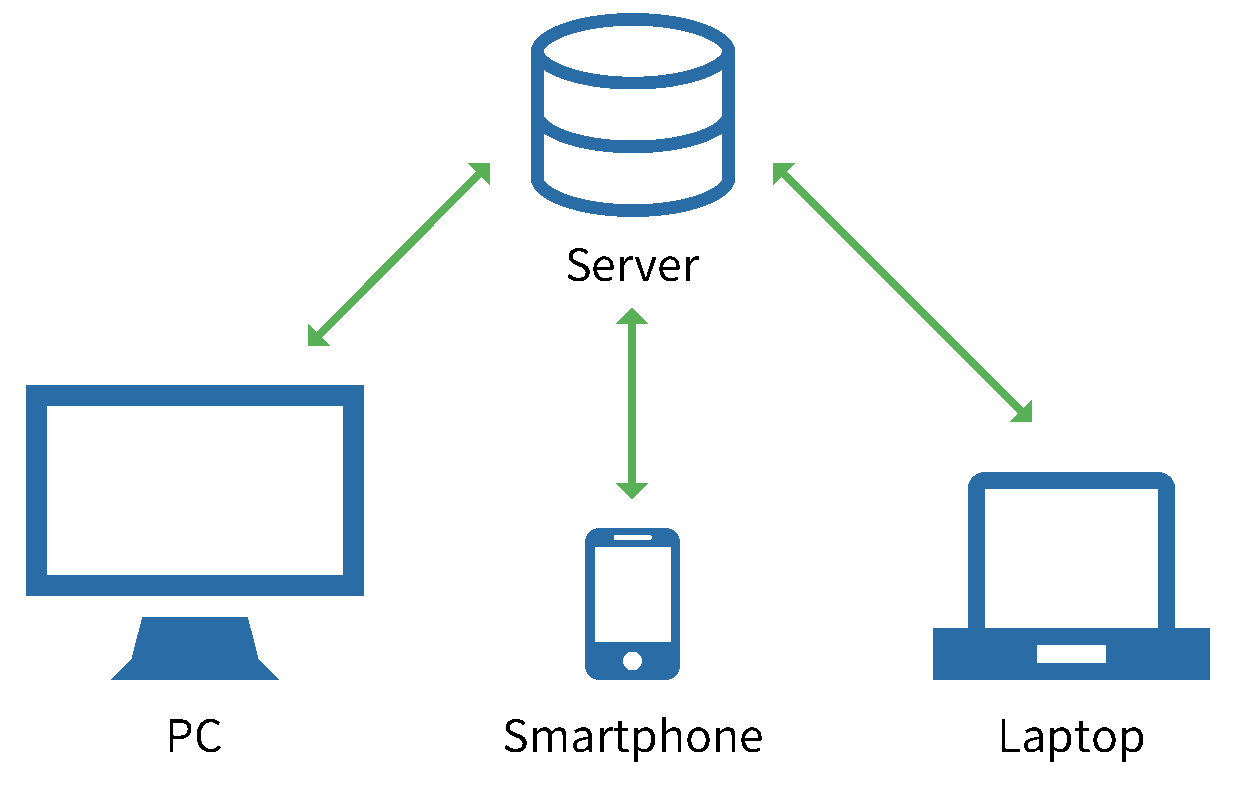
\includegraphics[scale=0.1]{img/Client_Server.png}
\caption{Client-Server architecture\cite{terms_2017}}
\label{fig:client_server_model}
\end{figure}

Having established the structure of the retail system regarding the separation of elements in tiers, a more in-depth analysis was performed to identify what architecture would fit best the client platforms. The chosen model for the components of both the web and the iOS applications was the Model View Controller architectural pattern. This ensured the logical separation of the user interface components used to present user specific information as View components, the data that provided the relevant information as Model elements and the actual logic of manipulating and when and how to display them as Controllers. This ensured a more robust and user-friendly structure of the application, also providing modularisation and control access, as well as clearly outlined rules of communication between components. In addition, the iOS applications implementation language is based on the Model View Controller design, encouraging the reuse of elements and also providing the means of further extending the application functionalities and design \cite{client-server_model_2017}. About the current solution's structure, all the major functions that a customer can execute (from managing their profile to navigation features) can be accessed through six view elements. Upon the initiation of an action, the respective view component will send a request to the central controller, which will perform the set of steps required for the completion of the task. This is achieved by manipulating the model components which incorporate the data elements, upon the modification of which the view elements will, in turn, be notified and changed. As a result, the established architecture for the retail system is the Client-Server design in combination with the Model View Controller pattern for the client tier as can be seen in Figure~\ref{fig:system_architecture}.\\

\begin{figure}[!ht]
\centering
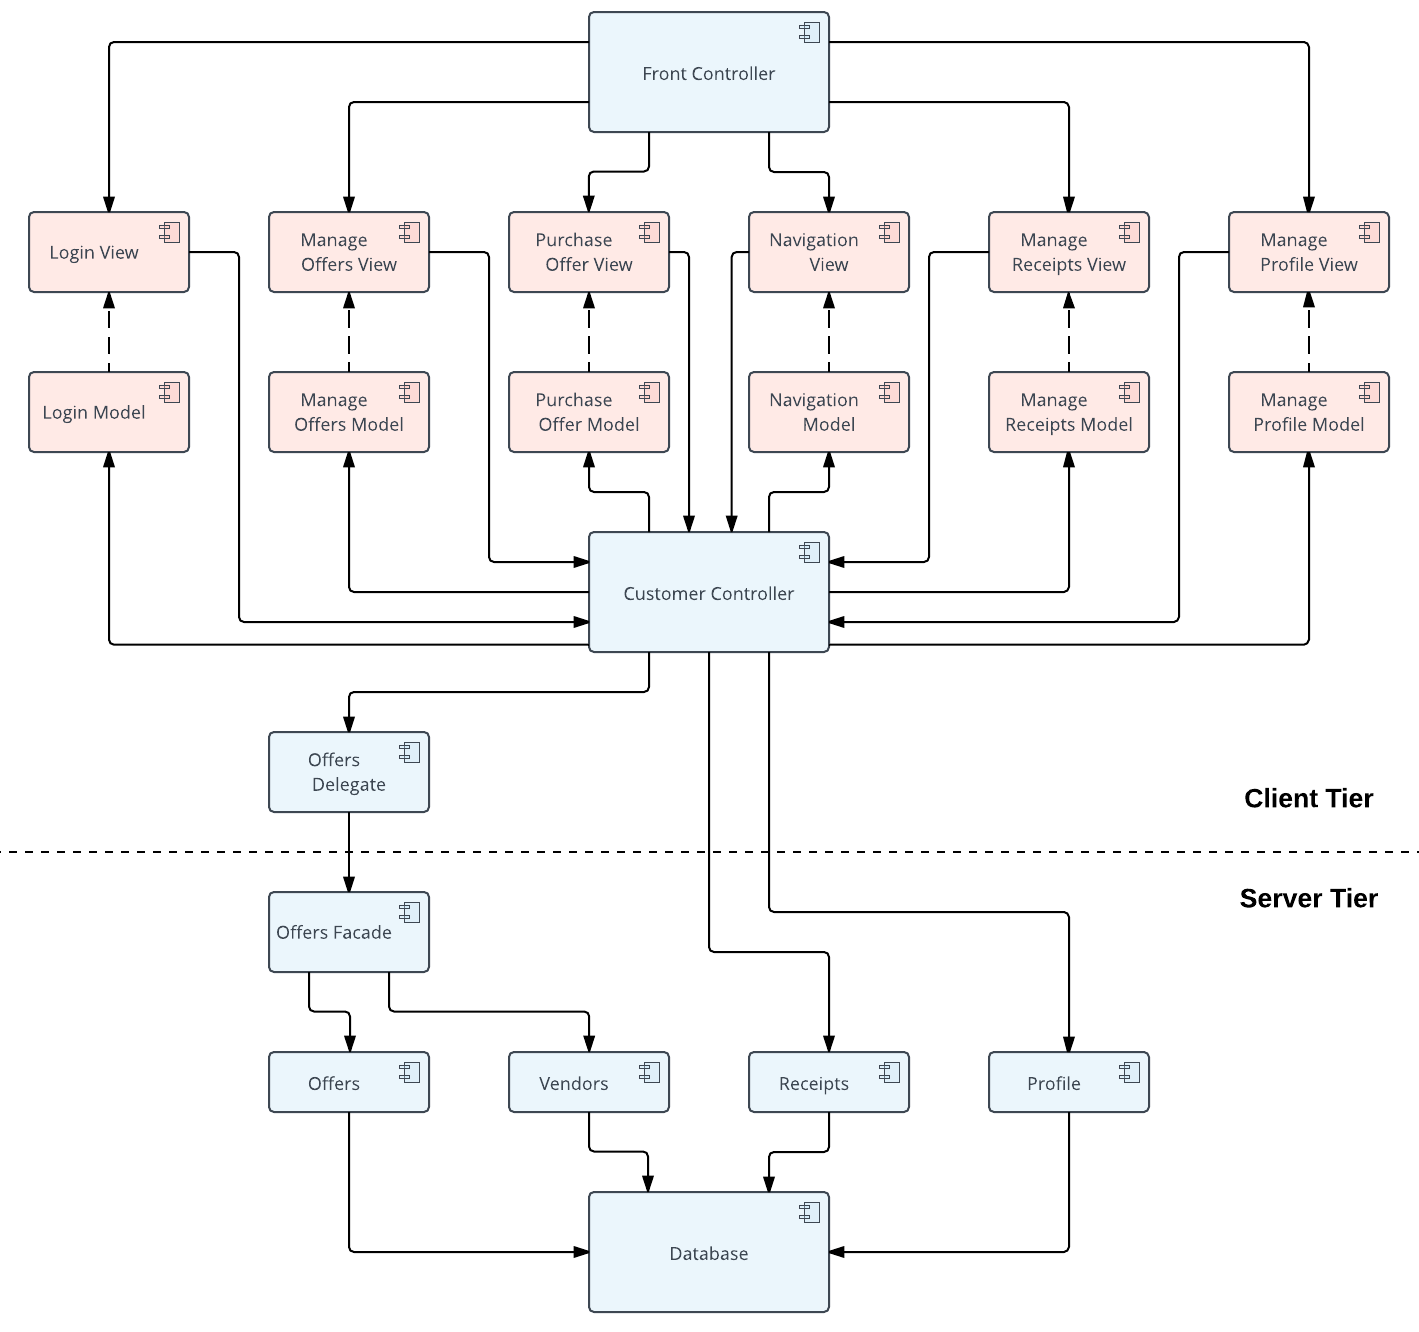
\includegraphics[scale=0.22]{img/System_Architecture.png}
\caption{Customisable system architecture}
\label{fig:system_architecture}
\end{figure}

\subsubsection{Design Patterns}

As the generation system's clients aim to use the software deliverable for large scale deployment, the retail system needs to provide robustness and high speeds in the communication between the client platforms and the server segment. To accommodate these requirements, some design patterns have been used, each targeting specific potential problems that might arise. These patterns provide further improvements concerning either speed or memory preservation and are general solutions identified for problems that have frequently appeared in software systems development throughout time. As a result, some improvements have been added to the system's Model View Controller, and Client-Server combined architecture in both the presentation and the business logic tier.\\

The first such structure used in the retail system's architecture modelling is the Front Controller design pattern, which aims to reduce the complexity of the navigation structure of the iOS or web platforms. Each view used for displaying information and detecting user intents in the client applications provides distinct functionalities specific to their segment of system logic. However, they share similar behaviour to accomplish their specific scopes, especially initial steps such as the authentication requirement and content retrieval. Through adding the Front Controller component as an intermediate interaction point with the views, the presentation applications seamlessly deal with handling errors and maintaining consistency in the navigation structure.\\

Another added presentation tier component is the Offers Delegate, which reflects the Business Delegate design pattern. This element has the purpose to reduce the number of connection points in between the two tiers, thus encapsulating the interaction in addition to providing modularity in the case of any business logic modifications. This approach leads to a decrease in the number of requests performed from the client side to server components, as well as providing an intermediate component which can perform mitigation regarding failed requests and also cache certain information, increasing the response speed and saving bandwidth. The identified segment of information that would be most accessed throughout the system's lifecycle regards the available offers.\\

The final improvement made to the architecture of the vendor solution was adding the Offers Facade component in accordance with the Session Facade design pattern. Similar to the Offers Delegate element, this model reduces the number of accesses to various components on the server layer. However, its primary purpose is to relieve the presentation tier of complex business logic operations that involve requesting services or information from separate server-side components. Acting as an interface for the client platforms, it helps reduce the dependency of the client tier on the remote components, as well as 
managing the retrieval of complex information from other business elements and performing the necessary operations locally on the server, providing a better end-user experience due to the increased speed.

\subsection{Implementation}

This chapter aims to present the processes involved in the implementation phase of the final solution. Having established the expected functionalities and the architecture, the next step was to initiate the actual creation of the software system. Following the timeline set in the planning phase of the project, the sequence in which the deliverables were created was designing the database, writing the server files, developing the iOS mobile application, creating the web platform, finishing with the generating system which required the completion of the other components. In addition to the functionalities implementation and platform specific constructs, this chapter will also present the graphical concepts and elements that form the user interface.

\subsubsection{Technologies and Tools}

The extensive number of components and functionalities considered by this project lead to the usage of various implementation technologies and development environments, as well as tools for the planning process. The reasons and motivation for choosing them are presented in the following section.\\

The database manipulation language selected for the data management of the customisable retail system is MySQL, an open-source software provided by Oracle that offers a substantial amount of functionalities. The main reason for which it was the best choice is that it is the primary solution for interacting with phpMyAdmin, a tool that provides great ease in working with data storage for server components. The combination of the two provides features necessary for the successful deployment of a software system such as the insertion, editing and deletion of data entries, as well as trigger functionalities that are executed automatically when previously established events arise. In addition, MySQL supports multiple concomitant connections with most of the existing development platforms without requiring too many resources \cite{schifreen_2010}.\\

The language of choice for writing the server components source code is PHP, a server side scripting language developed for web programming, as well as general usage \cite{runceanu_2014}. Using PHP ensured a seamless database connection process, being used exclusively in the data collection operations and the processing of the responses in the scope of forwarding only the relevant segments of business information. It has also been of use in the development of the client web pages for both of the systems of this project, providing the means of saving user relevant data persistently through creating sessions.\\

The development of the iOS application could only be achieved by using Xcode version 8.3.3, as Apple Inc. restrict the building process of any application to the usage of this development platform. However, this did not prove to be a limitation as the Xcode IDE offers a substantial amount of innovative features and functionalities, including a user interface generation system that provides ease in setting the boundary constraints and the customisation options of the graphical elements of an application. The chosen source code language for the iOS solution was Swift 3.1, a new version of the native object-oriented and functional programming language for iOS applications \cite{swift_2014}.\\

The design of the web pages included in both the retail system's web client platform and the generation system has been written using a combination of the HTML, CSS3 and JavaScript languages. HTML is standard for writing web pages as all the major browsers render the files into graphical interfaces by following the described structure. This is aided by CSS3, a styling language used to describe the graphical rules of rendering, from customisation options like colours and fonts to the placement restrictions of the visual elements. To further ease the development process, CSS3 provides modularity, being able to describe the rules of all the web pages in only one document. The web applications' functionalities and logic have been implemented through the use of JavaScript, a high-level language that enables programming the dynamic behaviour of websites\cite{schifreen_2010}.\\

Some external software solutions have also been used throughout the development process for providing the means of implementing the required features within the available amount of time. For example, the payment processing component used in both the web and iOS applications was developed by Braintree, a PayPal service that allows card validation and money transferring functionalities\cite{braintree}. Danijel Huis's HDAugmentedReality component is another already existing solution that allows presenting custom visual elements on the device's video camera screen when it is pointing in a previously established direction\cite{huis_2017}. Other external solutions helped in maintaining the graphical interface design throughout the whole system by providing the necessary elements for the iOS platform's interaction. A drop-down menu component has been used for offering the means of hiding buttons that are not frequently used, and a range slider element helped in the selection of the time interval filtering options. Also, some of these companies required active licenses for granting access to their services, such as Google Maps for the navigation components, Apple for the provisioning profile of the iOS application and Braintree for the payment processing.\\

Furthermore, a set of tools has been used for the planning, monitoring and controlling of the project progress. The Gantt chart presented in the planning process section was developed with the use of GanttPRO's project planning online app, providing the means of breaking down the RBS into work packages and arranging them with consideration to the duration, starting time and phase in which they were involved. This lead to the shaping of an estimated schedule for the development phase\cite{ganttpro_2017}. Apple Notes has been used for outlining the structure of the final report and for keeping the record of all implementation comments and variations\cite{notes_2017}. The choice of using this software was aided by the portability factor that helped to access the information from any personal device. Finally, the versioning control of the software package was done using the GitHub hosting platform\cite{github_2017}. This ensured a persistent copy of the source code files and the final report, as well as the means to go back to a previous version in the case of error.\\

\subsubsection{Database Templates}

As the retail system has to provide access to both global and user specific data for every client link established, whether it is from an iOS mobile application or a web browser, the need for a centralised data management system has been identified. To ensure reliable and atomic connections for requesting information from the global data source pool, databases have been used as the main component for storing and protecting the business particulars of the solution. Also, this enabled the possibility of further extending the functionalities of the platforms as databases have very scalable structures, as well as features for storing a large variety of elements\cite{what_is_database}. Also, the database can be programmed to perform specific tasks either at previously established times or upon their modification through trigger mechanisms, a feature useful in the case of the retail system for resetting the offer quantities and appointment time intervals from one day to another.\\

There are numerous classes of databases, varying in terms of how they perform the data storage. However, the most frequently used are the relational databases which organise the information in tables, providing modularity and many data access methods. To gather information stored in multiple tables, the allocation of a unique identification number for every entry is needed, which can also be referenced in other tables. Thus, tables can be joined based on the relationships established. This type of database has also been chosen for the retail system, as it provides all the required methods for accessing the centralised data. However, a poorly designed database structure can lead to hard to identify inconsistencies, resulting in the presenting of wrong information to the end user or even in receipt or credit storage mistakes, leading to financially related complications. To ensure that the structure designed for this project's solution in reliable, the database has undergone the normalisation process up until the third normal form, providing information integrity and preventing high levels of redundancy\cite{curcin_2016}.\\

\begin{figure}[!ht]
\centering
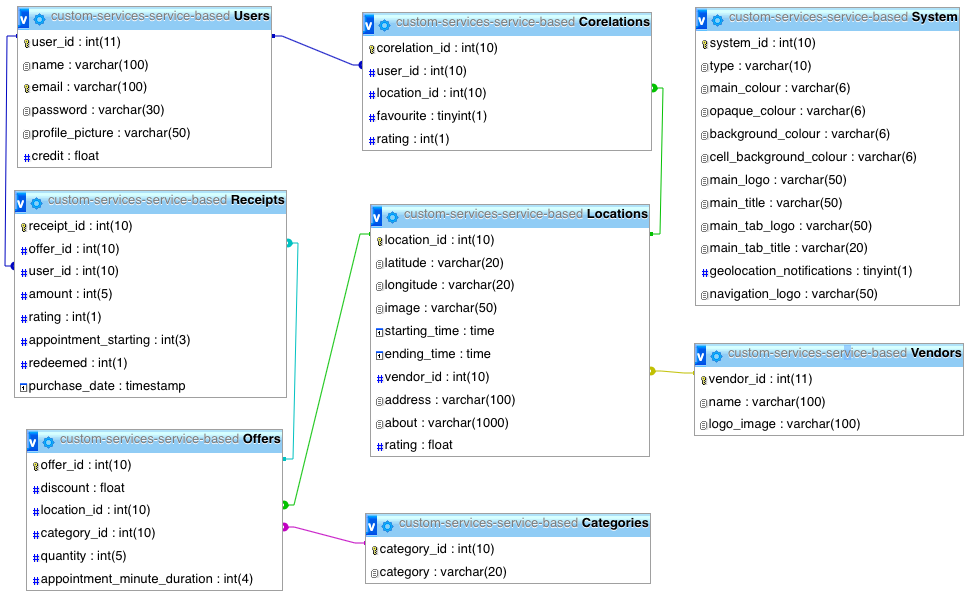
\includegraphics[scale=0.4]{img/database_structure.png}
\caption{Database template for service based systems with product categories}
\label{fig:database_structure}
\end{figure}

Creating the structure for the retail system's database started with the abstraction of business entities process undergone in the System Design section. The resulted platform independent model was then transformed into the relational database platform specific model by following a defined sequence of steps. Firstly, the subclasses were included in the parent elements to eliminate inheritance as this would have lead to redundancies in the database. This process was followed by providing unique identification key properties to all of the resulted classes to further restrict the possibility of having duplicate entries. These keys were then used to represent the relationships between entities by adding a foreign key field in the elements that needed a connection. Although, in the case of a many-to-many association, the relationship was reshaped by adding intermediary entities with references to both of the initial classes. Following this and the normalisation processes lead to the establishment of the database structure. However, the possibility of not having product categories and the three different types of retail systems regarded by the generating solution lead to the division of the database into six different templates. The structure of a service based retail system with product categories is presented in Figure~\ref{fig:database_structure}, as it is the only variation that includes all of the tables from the others.\\

All of the templates share the larger part of the structure as the aims of the possible systems still are the correlation of vendors and customers, the differences referring just to two characteristics of the solution. These designs include the Users table, which stores all the customer related information and credentials. However, the credit field is not present in the two variations that refer to location based retail systems, as no purchases can be performed. The Vendors table shows little information as the central part of the relevant data refers to the different locations described in the Locations section. However, multiple sites can belong to a single vendor, thus resulting in a foreign key association towards Vendors. The Correlations table has the purpose of maintaining the relations established between users and their favourite locales, each entry pointing towards the user and the selected location record. The Offers structure stores the special promotions available in their respective locations, including the discount (in the case of location based systems) or price in the field 'discount'. The Categories table is missing in three of the templates as the targeted products or services offers may not belong to various types. The product and service based systems provide the means of purchasing offers, thus storing the receipts in the table with the same name, where the availability is also recorded. The last segment is System, where the customisation options of the solution platforms are kept to be accessed by the client applications for redesigning the elements and filtering the available functionalities.\\

Having the possibility of triggering specific actions in the database at certain events was helpful in the case of service based solutions, as the quantity field is calculated automatically based on the appointment duration, the location's starting and ending times upon entering each record in the system. Another useful functionality that can be implemented in the future is setting the database to reset the quantity fields after the ending time of each location to restock the offers and appointments of the next day.\\

\subsubsection{Server Template}

Even though the main point of interaction between the retail system and the customers is on the iOS and web applications, having a reliable and well-designed server component is crucial for ensuring the best possible user interaction. The first step in reaching this goal was to rent server space from the DigitalOcean cloud service provider, ensuring that the system will be accessible throughout the implementation phase even from remote clients. Through this process and by configuring the server space with the LAMP stack provided the means to further scale the system in case of an increase in the number of users without having performance and storage space concerns. However, this feature targets only the retail platforms, as the server component of the generation system only has to provide the means for inputting data and generating the solution.\\

The transmission of information between the client and server tiers is achieved through HTTP, an application layer protocol that uses TCP to provide a more dependable connection for the transfer of data. The choice for this approach was straightforward as this is the primary communication method used in client-server architectures. The iOS and web applications perform HTTP requests to the server files which, upon the completion of their respective sets of operations, respond with any necessary information. Also, to limit the risks resulted from using this approach, an SSL security layer has been added to the server component, thus providing further encryption by using HTTPS requests.\\

The server tier of the retail system contains all the business logic required to provide the functionalities of the solution, acting as a middleware between the presentation applications and the database solutions. This was achieved through the component establishment and isolation performed in the architecture design stage described in the previous sections. As a result, the functionalities have been separated and tackled in different script files, each targeting specific data segments to manipulate and forward to the higher tier. One of the more extensive such components is 'service\_checkout.php', which performs all the validation and storage operations involved in the purchasing of service based offers. The necessary steps for achieving this interaction start with the validation of the offer and the available quantity, the existence of the user and the required credit amount, and the availability of the chosen appointment time interval. Next, the user details have to be updated with the new credit information, followed by reducing the offer's available quantity. Finally, a receipt is generated and inserted in the database, upon which the customer's new credit value and the identification number of the new entry are prompted to the client application for updating the visual interface with the new information. 

\subsubsection{iOS Mobile Application Template}

The core element of the customisable retail system is the iOS mobile app, which targets most of the potential customer segment. This component was developed with regard to the system requirements identified in the scoping process, as well as aiming to create a robust and proficient solution and to provide a high-quality user experience. Thus, the implementation phase was based upon the architecture established in the previous chapter, as well as following specific development guidelines and best practices. The functionalities include user session management, offers list filtering, map viewing based on current location, a purchasing system and augmented reality, therefore covering most features of a vendors and customers correlation application.\\

As the primary goal of the platform is to provide the means of visualising and choosing the best offers available, the three component views of the application's tabular structure target the filtering and management of discount products and services. This is achieved through using a table view element in the general and favourites offer sections and a map view for providing a more visual representation(Figure ~\ref{fig:iosmap} in the Appendix). The data source of all three segments is an array of offers received from the server tier after an initial request is performed upon the loading of the application. This array is saved in the persistent storage of the application to ensure having a backup version of the global list of promotions. The tables use variations of the array which are filtered based on category, the maximum distance from the current position, time intervals and availability, as well as sorted by proximity, rating score or discount value (the filtering options can be seen in Figure~\ref{fig:filters} in the Appendix). All these parameters can be modified by the user of the application to narrow down the list to the offers with the most potential. Also, as downloading all of the images beforehand can lead to unnecessary usage of storage space, they are retrieved only when presented on the screen. As such, one of the solutions implemented to reduce the latency produced by the cell renditions triggered by the scrolling gesture is caching the images to ensure that any latency will only affect the application once.  Another is using Swift's mechanism for reusing the cell view instances that have disappeared from the screen and changing just the content.  \\

The initial point of the platform is a front controller element which handles the navigation sequence. Thus, as the system targets only customers who are represented in the centralised database, the authentication process is initiated by opening the application. If user credentials are present in the persistent storage of the application, they are verified through a network request, and the main tabular view is displayed, thus reloading the user session. If the authentication fails or no information was previously stored, the login view is presented with the option of also registering. If a user wishes to change any personal details, the profile view offers such functionalities, as well as the possibility of crediting their account for product and service based systems. This operation implies entering the required amount and debit or credit card details, which are sent to Braintree \cite{braintree}, a payment validation system provided by PayPal. \\

This credit is used when an offer is purchased, the iOS application sending the request to the server which, upon acknowledging that the promotion is available, returns the receipt details. Service based systems operate on an appointment structure, in which case the application monitors their availability. As a result, if a location is fully booked, the purchasing button is disabled. The receipts resulted from bookings and purchases can be viewed in the Receipts section, where all of the user's previous orders are displayed in chronological order. When available, they are shown in the main colour of the system and can be presented to the vendors or, in the case of the receipts which have been previously redeemed, a rating button is enabled.\\

The functionality of showing notifications has also been implemented with two different scopes. Upon the creation of a receipt, the iOS application automatically triggers a notification event for thirty minutes before the redeeming is due. Also, if the system configurations allow it, geolocation notifications are set for all of the locations marked as a favourite. This was achieved by monitoring the current position using the iOS phone's location services and checking periodically if the customer has entered a one hundred meter radius area from the site of any favourite location. If so, an alert is presented to inform the user of the proximity. However, the application needs permission for using both the notification and the location services provided by the device.\\

\begin{figure}[!ht]
\centering
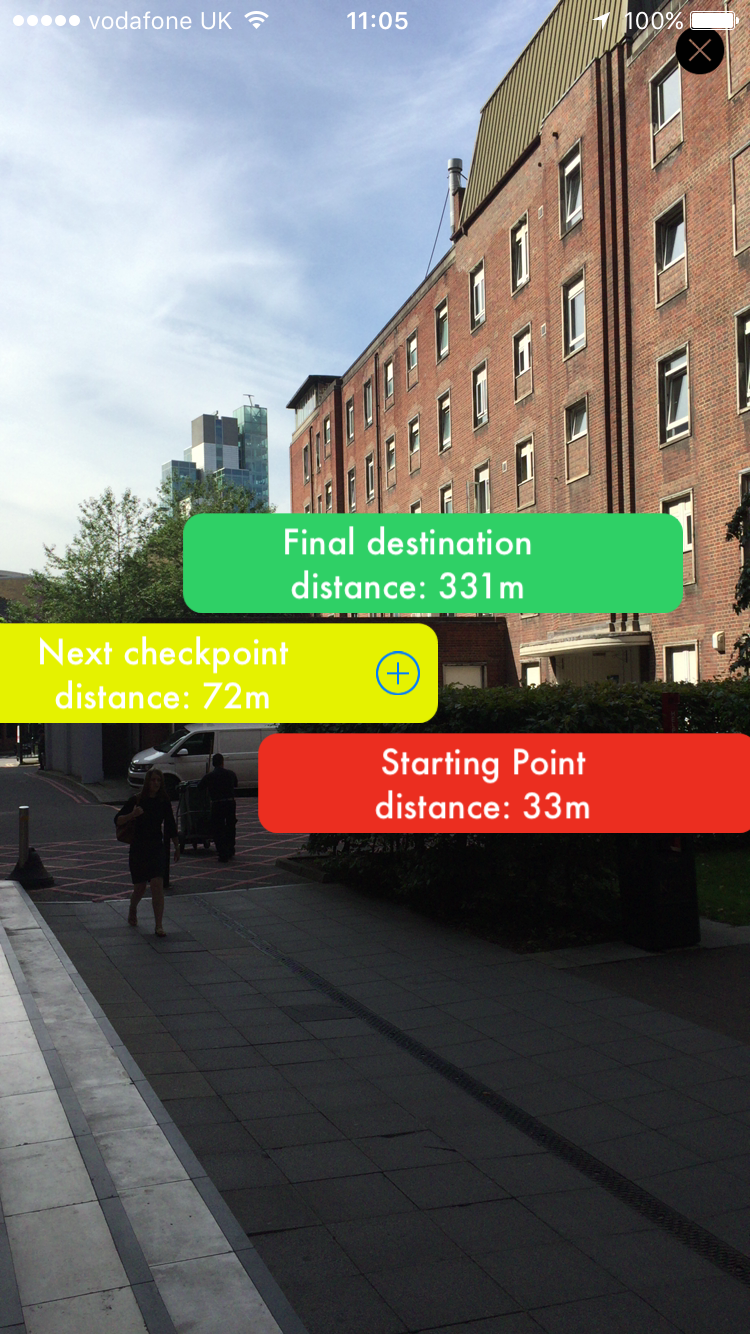
\includegraphics[scale=0.15]{img/ar.png}
\caption{Augmented reality checkpoint markers on the camera screen}
\label{fig:ar}
\end{figure}

The most interesting feature of the iOS application template is the possibility to provide navigation directions to any vendor location through augmented reality technology, as can be seen in Figure~\ref{fig:ar}. The implementation of this service involves requesting the step by step directions for the journey from Google Maps, parsing the JSON response for the retrieval of each checkpoint's coordinates, opening the camera for the augmented reality usage and presenting custom markers in the directions of the targeted points. An external solution has been used to accurately recognise when the device is pointed towards a particular point represented in three-dimensional coordinates. However, the navigation process consisting of the location monitoring for identifying when a checkpoint has been reached, and the sequence of displaying them were included in the implementation task on the mobile application. Permissions for accessing the camera and the location services are also required for this functionality. In the case that camera features are not allowed, the customers can choose between using either Google Maps or Apple Maps services in order to receive navigation directions towards the locations.\\

Finally, the feature that allows the iOS application to be called a template refers to the customisation options of the design and the selection from multiple visual elements based upon the system's type, as can be seen in Figure~\ref{fig:barbers_restaurants}. When the platform is started, an initial request is sent to retrieve the characteristics of the overall retail solution from the System entry in the database. Thus, the application detects the type, the presence of categories, the permission to enable geolocation notifications and the customisation parameters. The information is saved in the persistent storage and is accessed whenever a new view is triggered to appear on the screen, in order to set the label text values and system specific images, as well as to change the colours of the visual components.

\subsubsection{Web Application Template}

Most of the functionalities presented in the iOS mobile platform are also featured in the web application, except for the augmented reality navigation and receipts redeeming. The reason behind removing them from the web template is given by the platform limitations, as this component requires the usage of an internet browser. However, this environment provides better visualisation for the list of offers due to the larger size of the screen. \\

The initiation steps of the web application component are the same as in the mobile version, the front controller being represented by 'index.php', the root file of the platform. Upon accessing the website, the user session commences, and previously stored credentials are verified through a request to the server tier. If successful, an offer list is populated and the main view is presented. If not, the navigation is redirected towards a login and register page. In case of the occurrence of any major malfunction, an error page is rendered, and the navigation process must start from the beginning. \\

\begin{figure}[!ht]
\centering
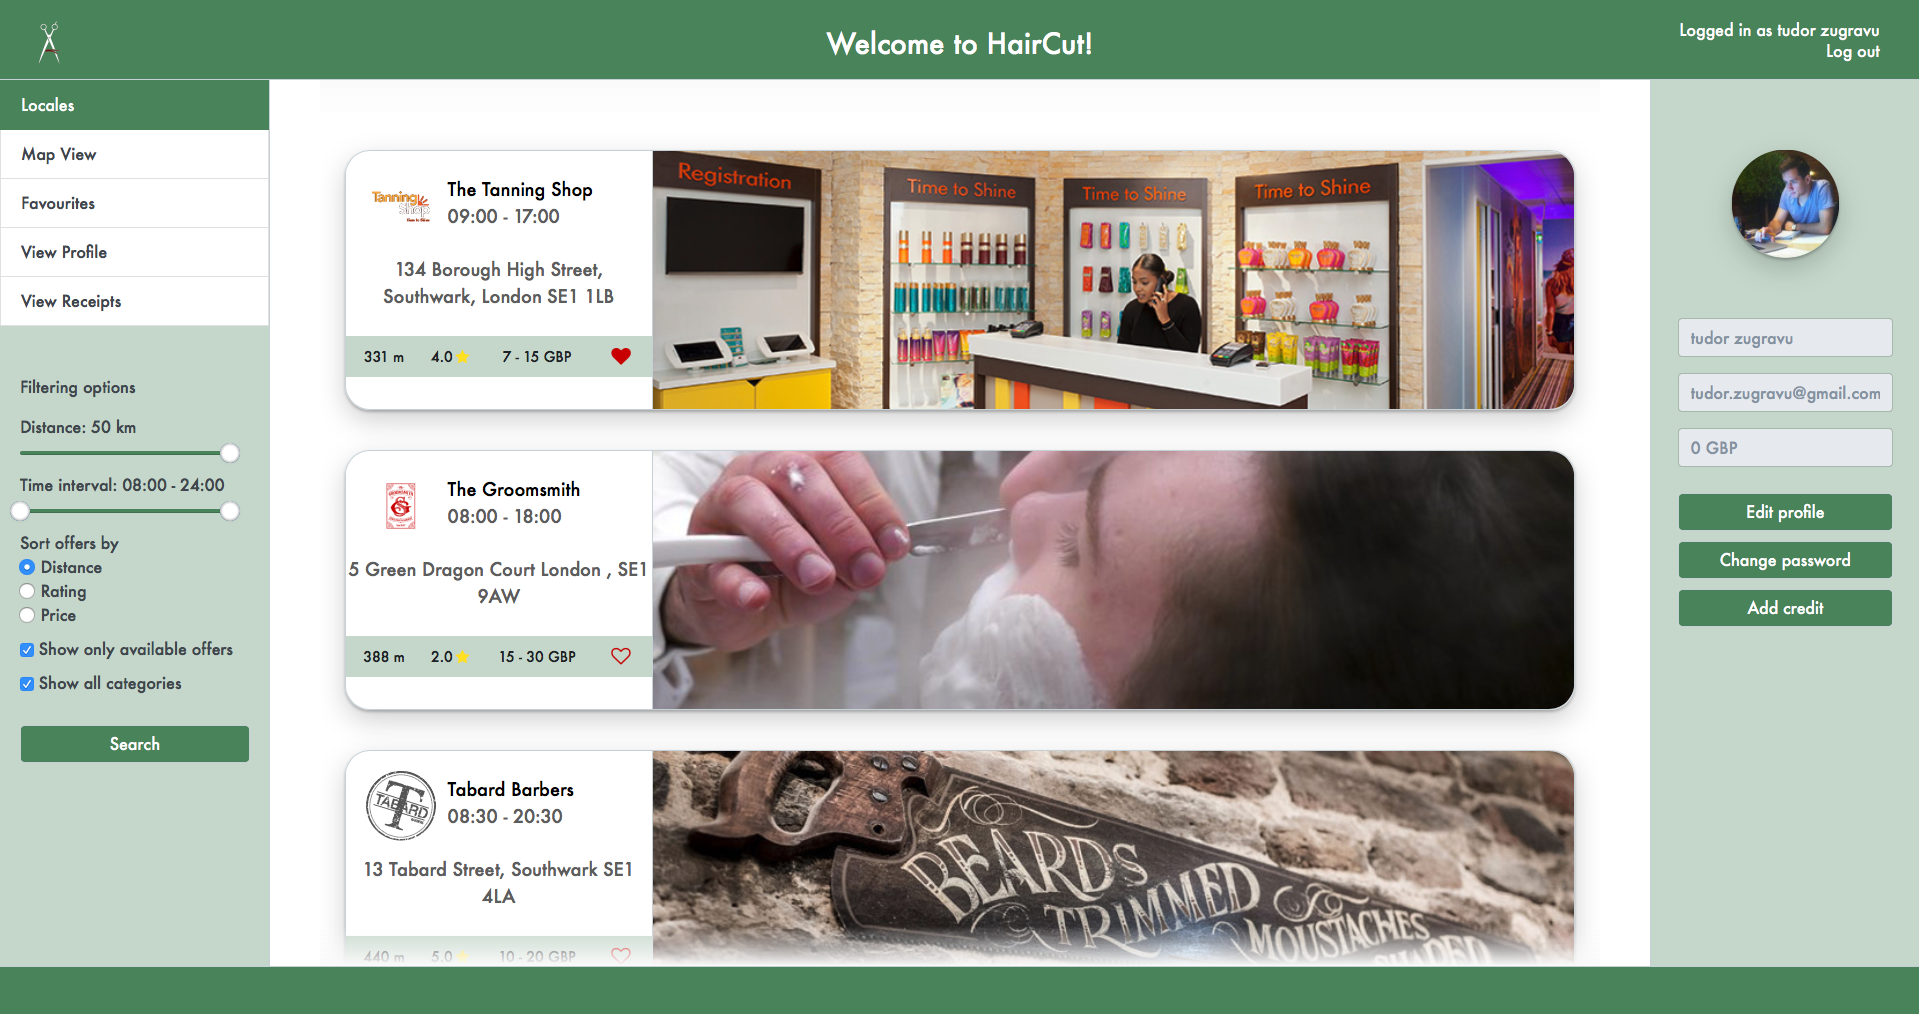
\includegraphics[scale=0.15]{img/barbers-web.png}
\caption{Barber shop variation of the web application}
\label{fig:barbers_web}
\end{figure}

The steps through which the information is acquired and manipulated are identical to the ones used in the iOS application, as both rely on network requests to the server and parsing of the responses. However, the presentation of the information is different due to the various structures of managing the graphical interface (Figure~\ref{fig:barbers_web}). Whereas the table view cells could be reused in the iOS solution, that feature is not present in the web application, possibly leading to heavily loaded pages. In contrast, the implementation process is simpler, as graphical elements that contain location specific information are just appended to the main view while iterating through the data source arrays. Also, the increase in screen size provides the means of presenting the filtering options and the profile details on the same page as the offer lists or map view, leading to a less complicated and possibly more intuitive workflow.\\

As in the iOS template solution, the current retail system characteristics are retrieved and saved in the user's session when the initial controller is accessed. They are used whenever there is a choice of elements that need to be presented based on the system type. The graphical customisation variables are also set through CSS classes, thus not having to change the appearance of every single element, as the elements are rendered based upon the classes of which they belong.

\subsubsection{Generation Platform}

The project's primary system was built last as it was dependent on the successful completion of all the other components. The first stage of its implementation was creating the client side web page through which potential clients could input their vendor system customisation requirements and perform the payment. The personalisation criteria for the solutions are the product's title, the name of the targeted consumer section, a set of colours for the graphical interface, the type of system, whether it be location, product or service based, the presence of categories and the choice of adding the geolocation notifications feature. If the payment process is complete, the generation of the solution is triggered on the server side.\\

The client platform of the main system sends the vendor platform customisation preferences of the client through a network request to its counterpart on the lower tier. The back-end operations for this segment are different from the retail server ones, as the focus is not on database queries and manipulation, but on the management of the various files that the retail system templates are comprised of. Upon the reception of a request, the system specifications are assessed to choose the best fit for the database structure out of the six different templates. The rest of the customisation options are formatted as an entry in the System table of the database and appended to the resulted file. It is archived together with the solution templates and a download link is provided to the client tier as a response.\\

The deployment process is described in a 'readme' text file attached to the generated archive, starting with filling in the solution server's IP address and the Google Maps API key needed for the augmented reality navigation system in the iOS client template. For the mobile platform to be released for commercial usage, the application also needs to be linked to an Apple versioning profile. The last step for this component's generation is to provide the folder with full permissions, as this is needed to build the iOS mobile application package. The server and web platform files need to be uploaded to the same IP address specified earlier to grant full access to any remote requests, and the database structure template should also be imported and populated with the system's targeted vendor and offer information. The last step is to locate the web application's configuration file and fill in the database name chosen beforehand, thus leading to a fully functional retail system.\\

\subsubsection{User Interface Design}

The main aspect that was taken into consideration while designing the visual elements of both the iOS and web application templates was maintaining consistency between platforms. This was ensured partially by the customisation criteria applied in both solutions. Also, the use of previously established design structures leads to cognitive recognition, thus providing a more simplified user interaction every time the platforms are accessed. Furthermore, the navigation sequences were simplified, and restrictions were enforced to prevent irregularities. For example, the navigation process of the iOS application works by pushing new views on top of the existing ones. As a result, if two pages have links to one another, going to and fro between the two views creates new instances over and over again, thus straining the memory and resulting in increased latency.\\

\begin{figure}[!ht]
\centering
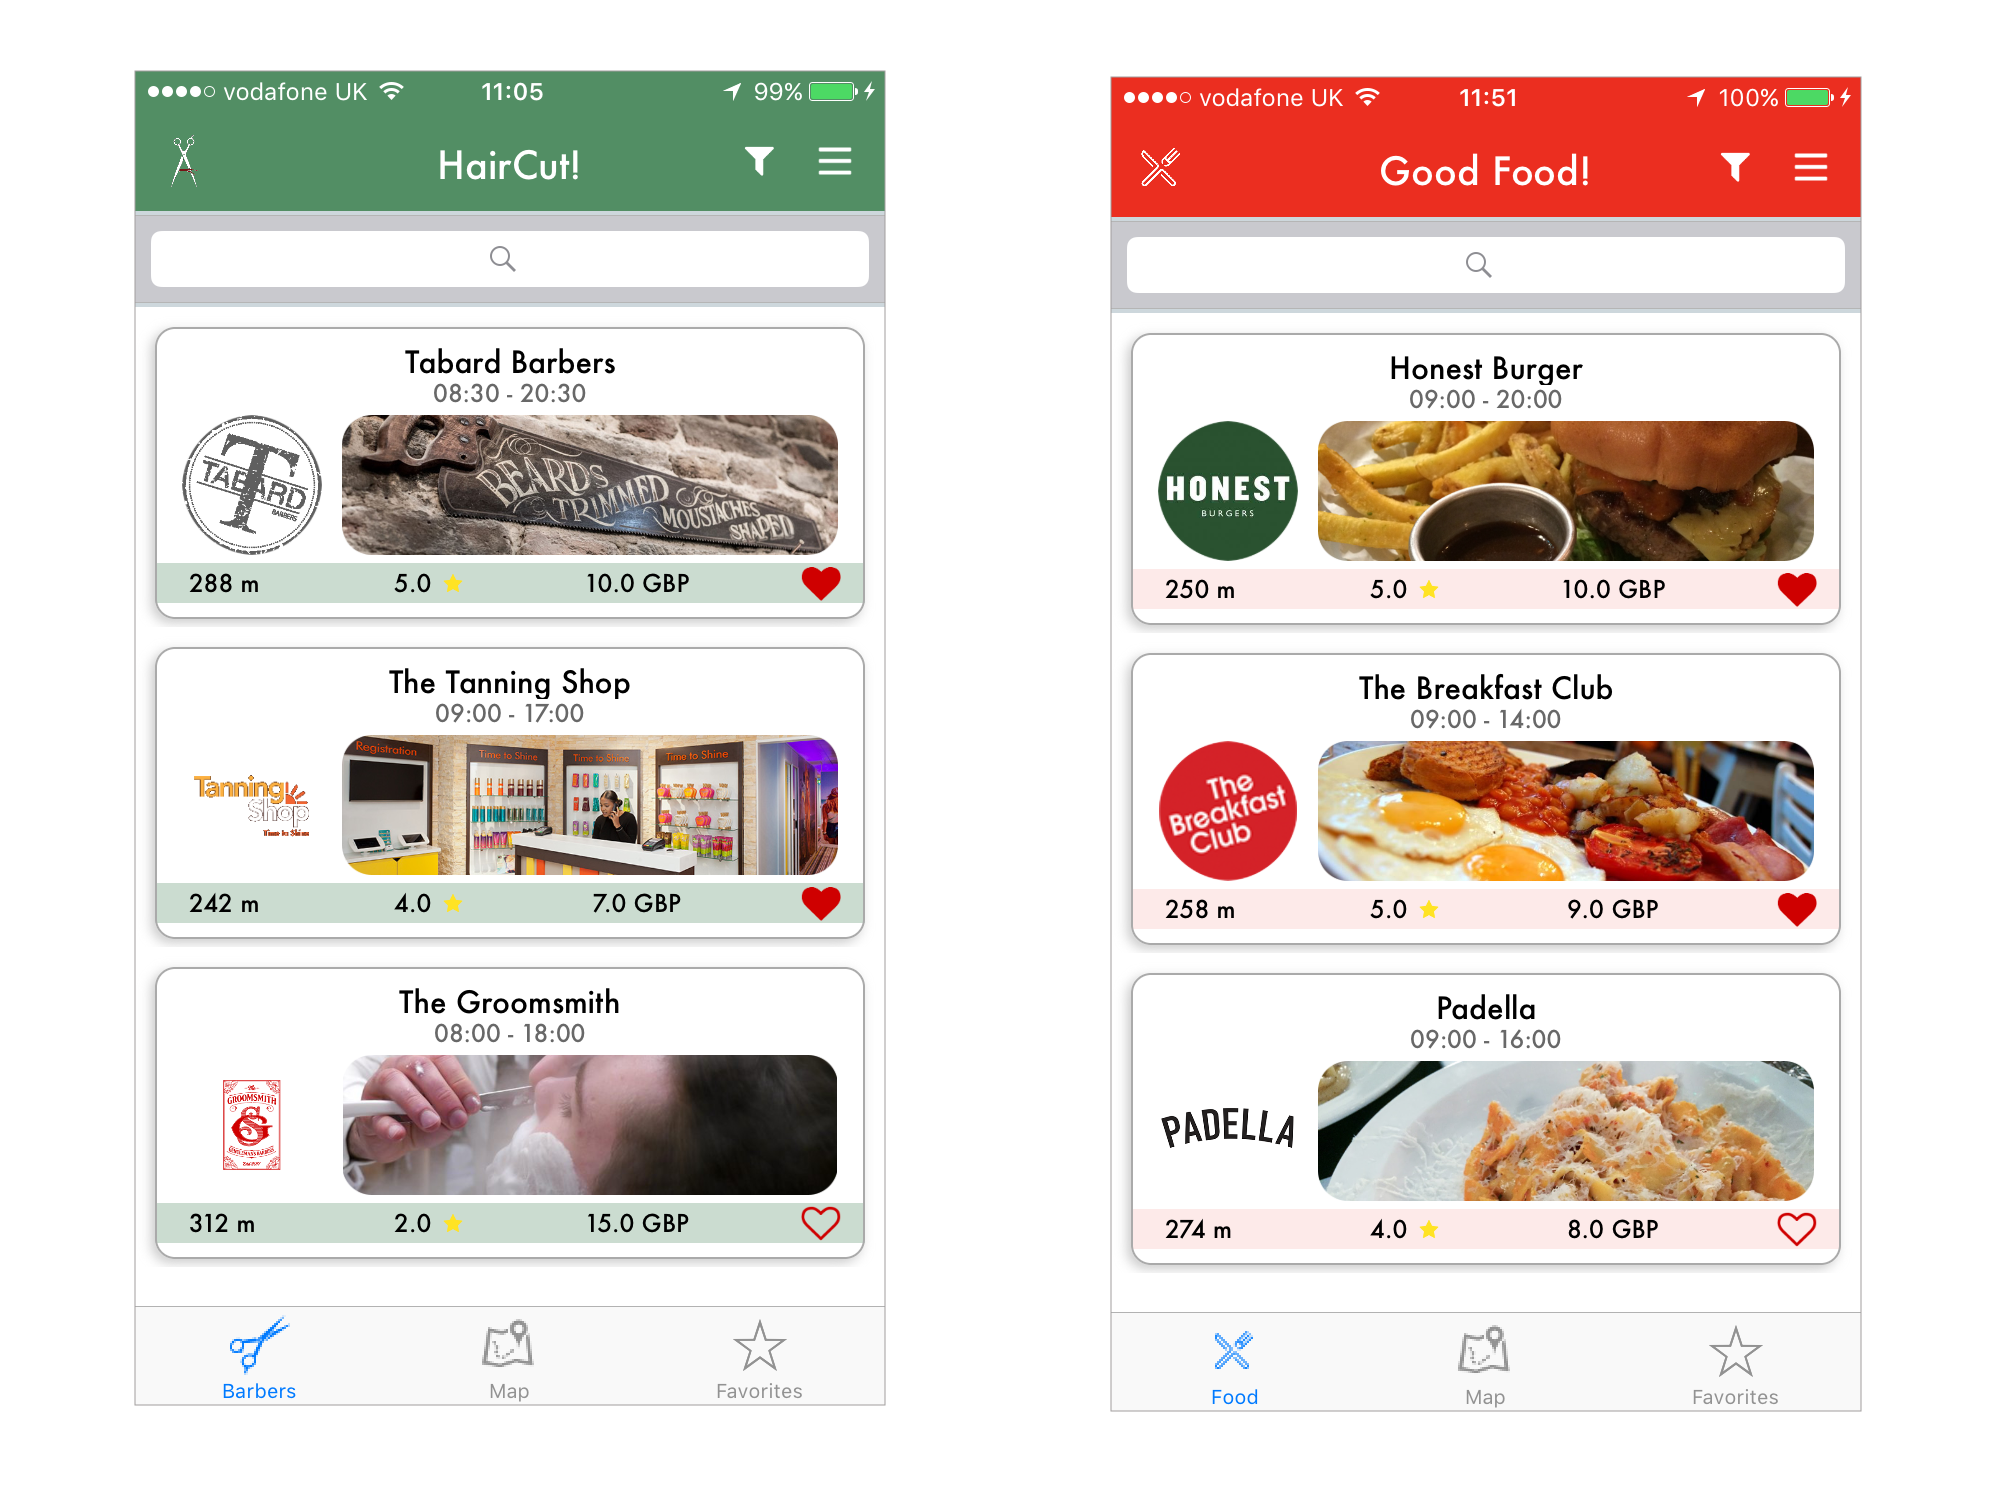
\includegraphics[scale=0.15]{img/barbers-restaurants.png}
\caption{Barber shop and restaurants targeted variations of the iOS mobile application}
\label{fig:barbers_restaurants}
\end{figure}

The customised solution generation implemented in this project implies adjusting the colour palette based on the client's preferences. However, the first version of the system does not allow choosing the position of the graphical elements on the screen. A previously established layout is provided, the design of which regarded the most strategic points of where the information should be displayed. As such, the only visual aspects that can be changed are the colours, the iOS application's tab bar item logo and the images of the platforms, as seen in Figure. To ensure that the layout rules applied to the pictures do not derange the visual aspect, constraints have been enforced on the images sizes uploaded by the client.\\

\subsubsection{Results and Evaluation}

The final solution's development was finished upon the completion of the generation platform, as all the template components have been created and their functionalities implemented before that. Also, the communication processes and the dependencies between them have been defined and applied while building the solution, thus resulting in a completely functional system. Performing an analysis of technical requirements of the system suggested that the results are satisfying. Both the iOS and web applications have an almost indistinguishable latency, except when retrieving the offers for the first time, as the images need to be downloaded. However, the caching feature solves part of having this additional waiting time, even though better algorithms should be used in future releases. The space allocated on disk needed for installing the iOS application is not small, this being a potential problem for the customers. The increased storage requirements are due to the Google Maps component, which is essential for the navigation steps and the map view. However, the dynamic retrieval of images and offer related information helps mitigate this solution by reducing the bundle size. From a user experience point of view, both the web and iOS templates can be considered efficient, customers being able to access any page seamlessly as the number of steps needed to reach any view has been considered when the navigation structure was designed. \\

In contrast, a limitation of the system is that both the client applications require an internet connection to operate. Storing the data persistently was considered, but as the information is very dynamic and can change in a matter of seconds, this solution was abandoned for this version. Another major limitation is that the server component was designed based on the LAMP structure, restricting the configuration possibilities. Similarly, the only present mobile solution is for the iOS operating system, confining the customer segment to only iPhone users, as well as adding the requirement of having a device running on the OS X operating system, which is needed for building the application. The last major system constraint is that the customisable retail solutions can only be location, product or service based and not any combination of the three, thus restricting the target offers as well as the customer basis. \\

The testing of the five template components was performed by considering every one of them as backboxes. Thus, some evaluation cases have been established including acceptance criteria based on the system specifications. As such, the functionalities tested number the authentication, register, user session, profile editing, adding credit, purchasing, redeeming and navigation features. This process pointed to the discovery of some of the limitations and performance issues. However, the acceptance criteria were met for the functionalities, thus indicating that a complete solution for the retail customisation system was created.








